%%%%%%%%%%%%%%%%%%%%%%%%%%
\chapter{INTRODUCTION} \label{chap:1}
%%%%%%%%%%%%%%%%%%%%%%%%%%
The chemical and biochemical processes that are essential to living systems take
place in aqueous environment. Water, the most abundant liquid on the Earth,
participates in the ecological cycle and acts as the essential element of life. 
Gases in liquid environment ~\citep{Hummer1998} is essential to predict and propose  its interaction with solids and then to seek their possible uses.

%%%%%%%%%%%%%%%%%%%%%%%%%%
\section{Methane  and various gases in water}
%%%%%%%%%%%%%%%%%%%%%%%%%%
\begin{sloppypar}
 Diffusion of gases like  CO, NO, N2, halogens, and smaller alkanes (methane, ethane, propane and n-butane)  are some of the most important phenomena that occur and play crucial role in inorganic, organic, medical and environmental domain of science. Nitrogen, the most abundant element in the atmosphere has many biological and physiological importance for the survival of organism in earth. N2 is the essential building block of biological compounds such as amino acids and proteins. Nitric oxide (NO) is one of the most important signal molecules in a living cell. It is considered as a signal molecule playing a specific role in intracellular and intercellular communication, involves in many physiological and pathological processes~\citep{hou1999}. It is a ubiquitous intercellular messenger in vertebrates, modulating blood flow, thrombosis and neural activity. NO was proclaimed molecule of the year in 1992~\citep{culotta1992no}. In 1998, Nobel Prize in physiology was awarded for the discoveries concerning NO as a signaling molecule in the cardiovascular system. The production of nitric oxide is also important for nonspecific host defense, helping to kill tumors and intracellular pathogens. The biological role of NO as an intracellular messenger molecule mostly depends on the diffusion of NO, which determines its effective concentration in the active cells. The charge neutrality of NO molecule is hydrophobic with respect to aqueous solution which facilitates its free diffusion. When NO molecule is added to aqueous solution, it does not dissolve but instead is excluded by water (H 2 O)~\citep{zhou2005molecular}.  Carbon monoxide (CO), on the other hand is toxic to humans and animals when encountered in higher concentration ~\citep{thompson2009carbon}. The study of these molecules is of great importance because of their impact in living beings. Diffusivity/mobility of ions in aqueous solutions is important in physical, chemical and biological systems e.g., ion channels in membranes and in many systems of interest to chemistry and chemical engineering. Estimation of  diffusion coefficients of the binary mixtures of smaller alkanes with water (H2 O) are important for the study and design of many geological~\citep{dutkiewicz2003}, petroleum~\citep{montel1993, De2001}  and chemical ~\citep{pedersen2001, Pratt1995} engineering and environmental ~\citep{taylor2000} applications. Light hydrocarbons are originated massively in the subsurface either from the decomposition of organic matter by biochemical and chemical processes \citep{claypool1983} or biogenic and thermogenic processes~\citep{strkapoc2011, hinrichs2006}, depending on the usual temperature and pressure conditions. Upon gathering they can migrate upwards, as a result of buoyant forces. If interstitial H 2 O is caught by the light hydrocarbons, either during the production or the migration stages, dissolution and subsequent diffusion will take place. In oceanic sediments the  migrating gases can encounter the hydrate stability zone (provided that the pressure and temperature conditions are appropriate), where they can remain trapped in the form of solid clathrate hydrates~ \citep{ginsburg1997}. If hydrate formation is not possible, eventually the migrating gas can reach the ocean floor. The competition between diffusion and  advection  in the H 2 O column will determine whether the light n-alkanes will eventually escape to the atmosphere ~\citep{mcginnis2006}. Such processes can have a significant effect to the global climate since methane (CH 4 ) is a strong greenhouse gas. Green house gases are supposed to be the main cause of {\it global warming} (the continuous increases in temperature of the earth) which has endangered natural creation and human life. Furthermore, the first four members of alkanes are also neutral analogs of amino acid side chain. Amino acid side chain analogs represent a natural test case for biomolecular interaction \citep{shirts2003,shirts2005solvation}. Methane is a simple molecule and the first member of saturated hydrocarbons, and  it is thus not surprising to know that it was one of the main components of the early Earth's atmosphere~\citep{franks2000}. In addition to this, it is found in the atmosphere of  some outer planets (Neptune, Uranus, Saturn) and their  moons (Titan - one of the moon of Saturn) in solar system as well as in outer space~\citep{Loveday2001a}. From an economical perspective, methane is becoming
increasingly important as a source of energy, and from a climatic perspective is an important greenhouse gas. The free energy of solvation represents a very important property for the thermodynamical description of a solution with impact in the chemical, biological, and pharmaceutical sciences. Alkanes are hydrophobic molecules, and as such its solubility in water is rather low, and alaknes molecules tend to aggregate when solvated in water. This behavior is more clearly exhibited by longer n-alkane
chains, which may be considered as polymers of methane. The diffusion, solubility or hydrophobicity of hydrocarbons (alkanes) in water is a basic consideration in many processes like processing of natural gases and petroleum~\citep{montel1993, kartsev1959}, understanding the tertiary structure of proteins, as well as the important role it plays as a driving force in a number of processes occurring within living cells~\citep{Privalov1988, kyte2006}. Here on Earth, methane is in contact with water
in many situations, and so it is important to understand the interactions between
these two molecules.  Therefore, although the solubility of methane in water may seem of rather limited importance, the correct description of the interactions between methane and water can be considered as a first step to improve our understanding of hydrocarbons and other more complex organic molecules in water. A second reason to study the behavior of methane in water is the formation of methane hydrates. Methane hydrates are crystalline solids, with non stoichiometric composition, which are formed when methane under pressure is cooled in contact with liquid water at temperatures around the melting temperature of water. Their presence in gas pipe-lines is considered, correctly, a major problem since they throttle and block the flow of gas causing enormous damage and expense. On a more positive note, it is thought that the amount of methane stored in the form of hydrates, typically in deep seas, is many times greater than that currently available from regular extractions~\citep{lerche2004, appenzeller1991}. 
\end{sloppypar}


Diffusivity data of the molecular diffusion of dissolved gases in liquid can provide important checks on any proposed theory or model of the liquid states. Also, diffusivities
of gases in liquid are important to engineers in gas-liquid mass transfer calculations and
correlations~ \citep{himmelblau1964}. Nitrogen, mostly an inert gas , is the most abundant particle in nature (78\%). The physiological exchange of inert gases, as well as measurement of pemeability
of tissues to inert gases, have emphasized the importance of precise measurements of the
diffusion coefficients of inert gases through liquids~\citep{smith1955experimental}. Nitrogen is the essential building
block of biological compounds such as amino acids and proteins. It diffuse in the soil from
environment and the plants incorporate it into amino acids production. As a negative
impact, nitrogen mix with oxygen in air to form nitrogen compounds (NO, NO 2 , N 2 O)
which then diffuse with rain water to result acid rain. Also this compounds result in
ozone layer depletion and green house effect~\citep{yung1976greenhouse}.
Nitrogen is used in nitriding process which is the diffusion hardening of steel in which
nitrogen is diffused into the surface steel. In this process nitrogen diffuse into the steel
and forms nitride alloys, and goes to a depth upto 0.65 mm~\citep{venugopalan2000effect}.
In underwater diving an inert gas like nitrogen is a component of breathing mixture
which is not metabolically active, and serves to dilute the gas mixture. Nitrogen can cause nitrogen narcosis and decompression sickness in the diver~\citep{rommel2006elements}.

Carbon monoxide, normally present in the atmosphere at a concentration less
than 0.001\%, is an odorless, colorless, and tasteless gas. It is readily recognized
for its toxic effects when encountered in higher concentrations though is also
produced in normal animal metabolism in low quantities~\citep{palali1997skin}.
Worldwide, the largest source of carbon monoxide is natural in origin, due to
photochemical reactions in the troposphere that generates about $5 \times 10^{12}$ kilograms per year. Other natural sources of carbon monoxide include volcanoes,
forest fires, and other forms of combustion~\citep{thompson2009carbon}. Besides the natural production,
some production is also due to vehicular and industrial emission.
Carbon monoxide (CO) is a very weak direct greenhouse gas, but has important
indirect effects on global warming. CO reacts with hydroxyl (OH) radicals in the atmosphere reducing their abundance. As OH radicals help to reduce the lifetimes of strong green house gases like methane, carbon dioxide, nitrous oxide, CO indirectly increases the global warming potential of the gases.
Carbon monoxide (CO) is a pollutant commonly recognized for its toxicological
attributes. One of the major causes of deaths in fires has been smoke toxicity. CO, a highly toxic combustion product, is one of the major component of smoke derived from fires, a primary cause of the lethality for smoke in fires. It is rapidly absorbed through the lungs and binds mostly to haemoglobin (Hb) and mildly to intracellular cytochrome oxidase. The affinity of CO to Hb molecule is
200-240 times more than the affinity of Oxygen to Hb. As a result the carboxy-haemoglobin level increases which limits the oxygen carrying capacity of the Hb
resulting cellular anoxia which leads to systematic and cutaneous manifestations
in pregnant woman~\citep{palali1997skin} 


Salts of monovalent ions are highly soluble in aqueous environment, and the solvated ions have important active roles in screening charge, moving charge, and also influencing the structure and dynamics of biomolecules such as nucleic acids and  proteins~\citep{auffinger2004, flick2013}. Given this, accurate modeling of biomolecular structure, dynamics, and function requires certain representative model of ionic interactions and mobile ions. Evaluation of the mobility of ions at infinite dilution and their dependence on ion size and the properties of the solvent is one of the classical areas of the study in physical chemistry. When an ion is placed in a polar medium, surrounding solvent is polarized due to the electric field of the ion. If the ion is displaced, the relaxation of the solvent polarization should take place to accommodate itself to the new position of the ion. The relaxation process is associated by an energy dissipation, and the corresponding force can be identified as the dielectric friction. The friction reduces with decreasing electrostatic field as the ion size increases ~ \citep{chong1999dynamics} . The diffusion of ions refers to the tendency of charged fragments of molecules (ions) to move from regions of high concentration to regions of lower concentration. The diffusion is a direct result of
the random thermal motion of the ions. The rate at which a particular ion species diffuses depends
on many factors, including the average speed of the ion, which in turn depends on its mass~\citep{atkins2006}.

\begin{sloppypar}
The structure and behavior of complex organic and biochemical systems may be examined at the molecular level using molecular dynamics and statistical mechanics techniques. On the other hand, methane is the simplest alkane molecule and can be a model structure to understand the process in protein folding and its denaturation ~\citep{Hummer1998}. In this context, understanding methane in different environments like, methane hydrates, porous carbon materials and liquid media, is the first step for methane related multidimensional practical applications. In the present work, we will discuss the structure and diffusion of N2, NO, CO in water, diffusivity and mobility of alkali ions (Na+, K+)  and halide ions (F-, Cl-, Br-, I-) in water and transport   properties of light alkanes (methane, ethane, propane and n-butane) in water, and free energy of solvation of the light alkanes in different aqueous environments, water and methanol. The solubility of various organic molecules such as drugs, vitamins and hormones is of
great physiological importance and we will be looking in substantial detail about the
solubility of various biologically important organic molecules. 
\end{sloppypar}


%%%%%%%%%%%%%%%%%%%%%%%%%%
\section{Alkanes  in solvent environment}
%%%%%%%%%%%%%%%%%%%%%%%%%%
\begin{sloppypar}
Hydrophobicity of non-polar molecules in water is characterized by low solubility of solutes and strong like-molecular attractive interactions \citep{Sharp1991, Scheraga1998}. It can also be defined by the aggregating property of hydrocarbons in water/aqueous-solutions where the water molecules are excluded by the hydrophobes~\citep{IUPAC1997}. Hydrophobicity mainly includes two aspects of the interactions; (i) the effect of solute particles on surrounding solvent molecules, defined by hydrophobic hydration, and (ii) the tendency of solute particles to aggregate, defined by hydrophobic interaction \citep{Raschke2001}. Because of hydrophobic hydration, water molecules make a spherical shell around the nonpolar solutes (methane for an example). On the other hand, solute particles and nonpolar residues in proteins aggregate to expose less surface area to water, which is related to hydrophilic interaction. Solvent perturbation in solute-solute (hydrophobic) interaction is one of the model systems of biological processes in protein- (or/and protein like molecules) structure, folding, functions and denaturation \citep{Gekko1998, Hwang2011}. It has also been observed that the strength and magnitude of hydrophobic properties are affected by the size and nature of the solute particles, and also the temperature and pressure of the solvent environment \citep{Makowski2009}.
\end{sloppypar}
 
Hydrocarbons are the major components of biological molecules (including proteins) and are widely considered to study hydrophobic processes. Proteins are made up of a long chain of amino acids with side-chain residues in different arrangements~\citep{Leach2001}. The interior of natural proteins is found to be occupied by the non-polar hydrophobic groups, which usually govern their structural stability. The surfaces, on the other hand, are covered by (charged) polar molecules, and play an important role in the formation/breaking of hydrogen bonding, a common process of solvent-solute interactions in hydrophobic effect. The hydrophobicity is also influenced by the variation in surrounding pressure - on increasing pressure water molecules are forced into the hydrophobic core and favor to denaturation \citep{Hummer1998}. Solvent induced interactions are noted in wider physical processes like surfactant coagulation, complexation, detergency and the formation of gas clathrates~\citep{Sobolewski2007}. 
 
The effect of temperature has been noted in protein structures. On rising temperature, the hidden nonpolar amino acids at the interior of proteins are exposed to water upon their unfolding/denaturation due to rising temperature \citep{Dill1990}. The enthalpic and entropic parameters are the indicators of hydrophobic effect, and thus finally play a vital role for protein folding and denaturation.
Nearby room temperature, temperature effects are mainly driven by the entropic contributions~\citep{Privalov1988}. For folded amino acids in water, where protein residues are more ordered with less exposed surface area, the entropic change is negative and the structure is favorable comparing to the removal of those molecules from water~\citep{Scott1950}. Dispersion interactions and point charge electrostatics are also important to identify the structural stability of side chains in aminoacids, and the same help to determine the nature of folding \citep{Raschke2001}. As the simplest hydrocarbon, methane is considered to model organic molecules within the solvent environment, which is important in biochemical processes~\citep{Dang1994}. Solvent induced solute-solute interactions, where hydrophobicity is the primary concern, can be described in terms of  free energy of solvation  as function of temperature \citep{Hotta2005, Li2007}.
 
\begin{figure}[h!]
\centering
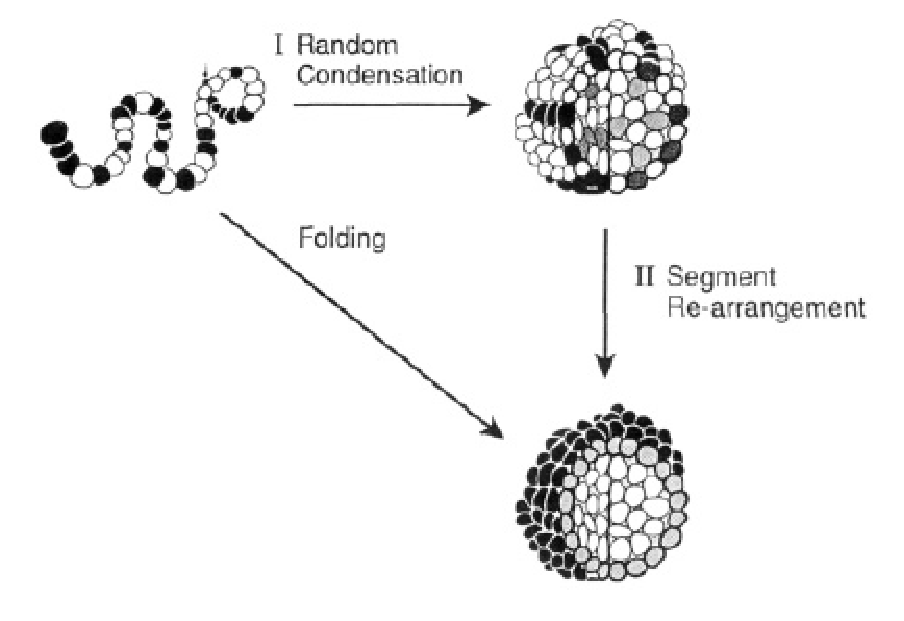
\includegraphics[width= 0.4\textheight]{Chapter1/Folded_non-folded.eps}
\caption[Random compactness of the chain and the rearrangement to more stable configuration.]{Process I represents random compactness of the chain and the process II represents the rearrangement to more stable configuration, where the nonpolar groups move into the core \citep{Dill1990}.}
\label{folded-nonfolded}
\end{figure}


 
Experiments lack the microscopic details to study the atomistic level of interactions. For example: X-rays diffraction requires the crystal environment and can not observe the disordered conformations \citep{Hwang2011}. Nuclear magnetic resonance (NMR) can identify intermolecular interactions, however, lacks high resolution of molecular parameters, their dynamics and the process of governing protein structure. The details, on the other hand, can be achieved through computational simulations like molecular dynamics \citep{Allen1989}. Computer modeling can thus be a source of information for the prediction of ongoing process in any system which can be verified by the following experiments \citep{Raschke2001}. Furthermore, limitations of computer simulations have been addressed in later modifications. Thermodynamic integration (TI) is a technique accommodated in GROMACS ({\it GROningen MAchine for Chemical Simulations}, a popular software for the method of molecular dynamics) which assists to find the free energy of solvation of different solutes in various solvent environments. We use BAR method~\citep{bennett1976} for finding the free energy of solvation of light alkanes in water and methanol. 

%%%%%%%%%%%%%%%%%%%%%%%%%%
\section{Rationale of the study}
%%%%%%%%%%%%%%%%%%%%%%%%%%

Diffusion is important to organisms because it is the process by which useful molecules enter the body cells and waste products are removed. Digested food molecules (amino acids, glucose) move down a concentration gradient from the intestine to the blood. Diffusion happens in  plants, for example, it explains the movement of carbon dioxide in leaves. Diffusion plays key role in the intermixing of gases and liquids, permeation of atoms or molecules through membranes,
evaporation of liquids, drying of timber, doping silicon wafers to make semiconductors
devices, transport of thermal neutrons in nuclear power reactions, chemical reactions.
The knowledge of diffusion is very important for scientists who design materials for
elevated temperatures and for engineers who build equipment for operation at such
temperatures.

The diffusivity and  solubility of light alkanes in water and their mixtures are of vital importance to the gas and petroleum industries. Preventing corrosion and hydrate crystal formation in subsea and terrestrial pipelines are examples of operating and safety problems, which require a precise knowledge of water content in hydrocarbons. Given the importance of the subject, a large number of results can be found in the literature. However, significant disagreement is found between these results, surely reflecting the difficulty of these measurements.


Methane in hydrates are important because of their dominant occupancy in nature. As a major component of natural gases, and less pollutant hydrocarbon than conventional sources like oil and gases, stability of methane in the conditions of natural occurrence is important. For the practical purpose
like for on-board applications, on the other hand, effective storage media are demanding. Since methane-methane interactions are affected by the environment where they sit on, similar to proteins in human body, the perturbation of liquid media on gaseous methane  are to be understood. Besides the dominant presence of methane in nature, it is beneficial over the conventional petroleum oil and fossil fuels because of its higher energy density and less emission of carbon on burning. The conventional techniques of storing natural gases as well as other energy carrying gases need either very high pressure with very low temperature and are not efficient due to space, safety and economy related perspectives. 



Solubility, lack of solubility and other solvation properties of atoms, molecules and ions in aqueous
solutions play a crucial role in biological processes and industrial applications. Methane and other light alkanes  interactions in different liquid media can be a model research to understand the hydrophobic interaction in atomistic level. Understanding of such interactions is important in biological processes including protein folding and its denaturation. Biological processes, such as signaling, gene regulation, transcription, translation, et cetera govern the cell growth, cellular differentiation, fermentation, fertilization, germination, etc. in living organisms. Chemical processes, such as oxidation, reduction, hydrolysis, nitrification, polymerization, and so forth underpin biological processes. Physical processes, particularly solvation, are involved in all the aforementioned chemical and biological processes. Therefore, a prerequisite for the understanding of chemical and biological processes is to study the solvation process.

%%%%%%%%%%%%%%%%%%%%%%%%%%
\section{Objectives of the study}
%%%%%%%%%%%%%%%%%%%%%%%%%% 
Transport  properties (diffusivity)  various gases, like NO, CO, O2,  methane and other light alkanes, and some alkali and halide ions in water are studied  over a wide range of temperatures. This thesis is focused on the following main  objectives:

\begin{enumerate}[(i)]
% % % % % % % % % %
\item We intend  to study the structural and transport properties of nitric oxide in water and alkali ions (Sodium  and Potassium ion) and halide ions (fluoride, chloride, bromide and iodide) in water. Molecular dynamics (MD) simulation comes in handy for understanding the properties of assemblies of atoms or molecules in terms of their structure and the microscopic interactions between
them. This serves as a complement to conventional experiments, enabling us to learn
something new, something that cannot be found out in other ways. 

\item We intend to go through the temperature dependence of structure and   transport properties of light alkanes (methane, ethane, propane and n-butane) in water at constant atmospheric pressure.   

\item We intend to study  the thermodynamic property,  specially free energy of solvation of light alkanes in  different solvent environments,  water and methanol. Bennett Ratio Method (BAR)implemented  in GROMACS helps to calculate free energy of solvation of light alkanes in different solvent environments. This study is useful for understanding the biomolecular interactions in living cells. 
\end{enumerate}
%%%%%%%%%%%%%%%%%%%%%%%%%%
\section{Organization of the thesis}
%%%%%%%%%%%%%%%%%%%%%%%%%%
The structure of this thesis is organized as follows: 
\begin{enumerate}[(i)]
\item In chapter 2,  we shall discuss the available literature related to the present work. The chapter is named as Literature Review, which aims to prepare the required background and justify the objectives of the current work.

\item We present the theoretical background, necessary formulas and algorithm that we have used during the entire work in Materials and Methods (Chapter 3). Basic introduction  molecular dynamics (MD) simulations with some special features including the systems under study are discussed in the chapter. 

\item Chapter 4 presents a comprehensive study on transport and structural properties  of the studied systems. Section 4.1 introduces the background for the whole chapter. Section 4.2 deals with the structural and transport properties of methane and various gases in water at different temperatures.  In section 4.3, we present and discuss the diffusivity and mobility of alkali and halide ions in water. The findings of the free energy of solvation of light alkanes in different solvent environments; water and methanol are discussed in section 4.4.

\item The inferences and possible extension of the present work are collected in Chapter 5. The chapter is named as ``Conclusions and Recommendations''. ``Summary'' is noted in chapter 6. Finally the references are enumerated  before closing this PhD thesis project. 
\end{enumerate} 


